\documentclass[border=6pt]{standalone}
\usepackage[T1]{fontenc}
\usepackage{lmodern}
\usepackage{amsmath,amssymb,bm}
\usepackage{xcolor}
\usepackage{tikz}
\usetikzlibrary{arrows.meta,positioning,fit,backgrounds,calc}
\definecolor{swinc}{HTML}{2166AC}
\definecolor{cnnc}{HTML}{1B7837}
\definecolor{decc}{HTML}{E66101}
\definecolor{botc}{HTML}{B2182B}
\definecolor{headc}{HTML}{762A83}
\newcommand{\code}[1]{\texttt{\detokenize{#1}}}
\begin{document}
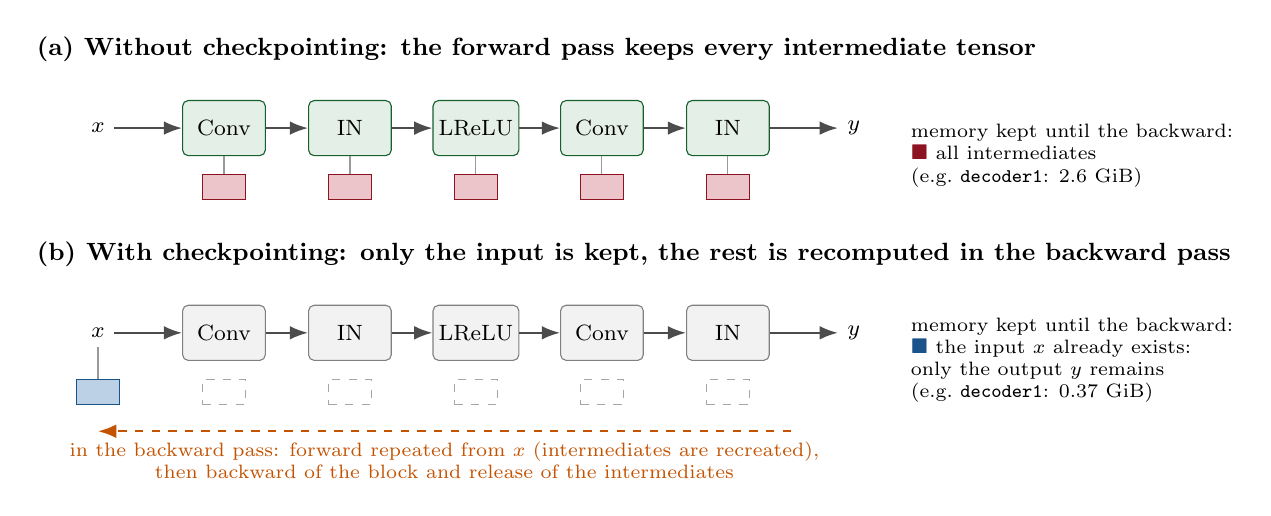
\begin{tikzpicture}[
  font=\footnotesize, >=Latex,
  op/.style={draw, rounded corners=2pt, minimum height=0.7cm, minimum width=1.05cm, align=center, inner sep=2pt, fill=cnnc!12, draw=cnnc!80!black},
  saved/.style={draw=botc!80!black, fill=botc!25, minimum width=0.55cm, minimum height=0.32cm, inner sep=0pt},
  kept/.style={draw=swinc!80!black, fill=swinc!30, minimum width=0.55cm, minimum height=0.32cm, inner sep=0pt},
  ghost/.style={draw=black!35, dashed, fill=white, minimum width=0.55cm, minimum height=0.32cm, inner sep=0pt},
  arr/.style={->, thick, black!70}
]
\node[font=\small\bfseries, anchor=west] at (-0.9,1.0) {(a) Without checkpointing: the forward pass keeps every intermediate tensor};
\node (x1) at (0,0) {$x$};
\foreach \i/\t in {1/Conv,2/IN,3/LReLU,4/Conv,5/IN} {
  \node[op] (a\i) at (1.6*\i,0) {\t};
  \node[saved] (s\i) at (1.6*\i,-0.75) {};
}
\node (y1) at (9.6,0) {$y$};
\draw[arr] (x1) -- (a1); \draw[arr] (a1) -- (a2); \draw[arr] (a2) -- (a3); \draw[arr] (a3) -- (a4); \draw[arr] (a4) -- (a5); \draw[arr] (a5) -- (y1);
\foreach \i in {1,...,5} \draw[black!40] (a\i) -- (s\i);
\node[anchor=west, align=left, font=\scriptsize] at (10.2,-0.35) {memory kept until the backward:\\ \textcolor{botc!80!black}{$\blacksquare$} all intermediates\\ (e.g.\ \code{decoder1}: 2.6 GiB)};

\begin{scope}[yshift=-2.6cm]
\node[font=\small\bfseries, anchor=west] at (-0.9,1.0) {(b) With checkpointing: only the input is kept, the rest is recomputed in the backward pass};
\node (x2) at (0,0) {$x$};
\node[kept] (k) at (0,-0.75) {};
\draw[black!40] (x2) -- (k);
\foreach \i/\t in {1/Conv,2/IN,3/LReLU,4/Conv,5/IN} {
  \node[op, fill=black!5, draw=black!50] (b\i) at (1.6*\i,0) {\t};
  \node[ghost] (g\i) at (1.6*\i,-0.75) {};
}
\node (y2) at (9.6,0) {$y$};
\draw[arr] (x2) -- (b1); \draw[arr] (b1) -- (b2); \draw[arr] (b2) -- (b3); \draw[arr] (b3) -- (b4); \draw[arr] (b4) -- (b5); \draw[arr] (b5) -- (y2);
\node[anchor=west, align=left, font=\scriptsize] at (10.2,-0.35) {memory kept until the backward:\\ \textcolor{swinc!80!black}{$\blacksquare$} the input $x$ already exists:\\ only the output $y$ remains\\ (e.g.\ \code{decoder1}: 0.37 GiB)};
\draw[->, thick, decc!85!black, dashed, rounded corners] (8.8,-1.25) -- (0,-1.25) node[pos=0.5, below, font=\scriptsize, text=decc!85!black, align=center] {in the backward pass: forward repeated from $x$ (intermediates are recreated),\\ then backward of the block and release of the intermediates};
\end{scope}
\end{tikzpicture}
\end{document}
